\chapter{Arhitektura i dizajn sustava}

		Glavni dijelovi arhitekture sustava su web preglednik, web poslužitelj i baza podataka.  
		
		Web preglednik omogućuje korisniku da pronađe određenu stranicu. Njegova funkcija je prevođenje stranica u svima razumljiv sadržaj. Neki od popularnih web preglednika su Google Chrome, Safari, Microsoft Edge, Opera. 
		
		Web poslužitelj je softverski program koji ima zadatak da pohranjuje, obrađuje i dostavlja klijentima web stranice. Komunikacija između web preglednika i klijenta odvija se HTTPS protokolom. 
		
		Programski jezik koji smo odabrali za implementaciju ove web aplikacije je radni okvir Spring Boot koji koristi višeslojnu arhitekturu. Spring Boot slijedi slojevitu arhitekturu u kojoj svaki sloj komunicira sa slojem neposredno ispod ili iznad njega. Postoje četiri sloja u Spring Boot arhitekturi, a to su: 
		
		\begin{packed_item}
			\item \textbf{Prezentacijski sloj} (engl. \textit{Presentation Layer}) - Ovo je najviši sloj arhitekture. Sastoji se od front-end dijela aplikacije. Obrađuje HTTP zahtjeve, provjerava autentičnost zahtjeva te pretvara JSON parametar u Java objekt. Nakon što provjeri autentičnost zahtjeva, dalje ga prosljeđuje poslovnom sloju.
			\item \textbf{Poslovni sloj} (engl. \textit{Business Layer}) - Ovaj sloj obrađuje svu poslovnu logiku te je zaslužan za autorizaciju i validaciju.
			\item \textbf{Sloj postojanosti} (engl. \textit{Persistence Layer}) - Sadrži svu logiku pohrane te prevodi poslovne objekte iz i u bazu podataka.
			\item \textbf{Sloj baze podataka} (engl. \textit{Database Layer}) - Može se sastojati od više baza podataka. Zaslužan za provođenje CRUD (engl. \textit{Create, Read/Retrieve, Update and Delete}) operacija.
		\end{packed_item}
	
		\begin{figure}[H]
			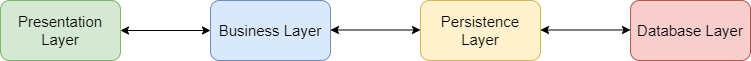
\includegraphics[scale=0.57]{slike/slojevi.png}
			\centering
			\caption{Slojevi Spring Boota}
			\label{fig:slojevi}
		\end{figure}
	
	\eject
	
		Komunikacija u Spring Bootu prikazana je na slici \ref{fig:flow}. Ona započinje kada klijent postavi HTTPS zahtjev koji se dalje šalje nadgledniku. Nadglednik mapira taj zahtjev i obrađuje ga. U sloju usluge obavlja se sva poslovna logika. Spring Boot izvodi svu logiku nad podacima baze podataka koja je preslikana u klasu modela putem Java Persistance biblioteke. U posljetku, ako nije došlo do pogreške, Java Spring Boot stranica se prikazuje klijentu.
				
		\begin{figure}[H]
			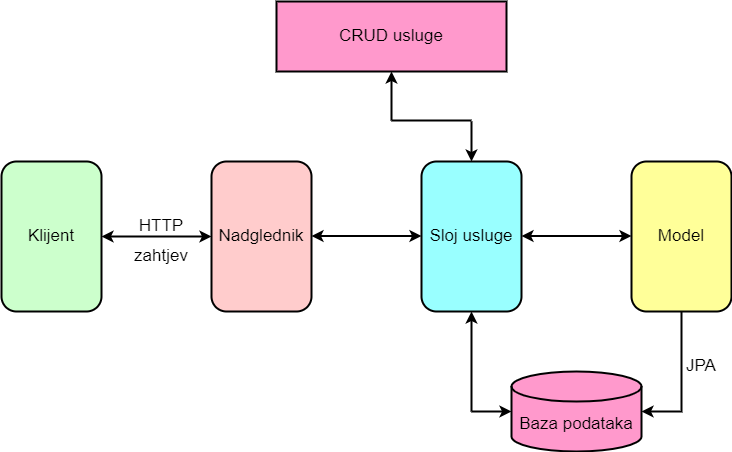
\includegraphics[scale=0.57]{slike/flow.png}
			\centering
			\caption{Komunikacija u Spring Bootu}
			\label{fig:flow}
		\end{figure}
	
		Uz Spring Boot koristili smo React koji je JavaScript biblioteka za izradu korisničkih sučelja. Primarna svrha Reacta je omogućiti razvojnom programeru stvaranje korisničkog sučelja koristeći čisti JavaScript.
		
		Kao razvojne okoline koristili smo IntelliJ IDEA za rad sa Spring Bootom te Visual Studio Code za rad u Reactu. 
		
				
	\eject
	
		\section{Baza podataka}
		
			Za potrebe aplikacije Sinappsa koristit ćemo relacijsku bazu podataka. Osnovna jedinica baze je relacija koja se definira svojim imenom i skupom atributa. Baza podataka pomaže u pohrani, izmjeni i dohvatu podataka koji su nam potrebni za obradu zahtjeva. Baza podataka aplikacije Sinappsa sastoji se od sljedećih entiteta:
			
			\begin{packed_item}
				
				\item Korisnik
				\item Profil
				\item Kolegij
				\item Smjer 
				\item Kategorija
				\item Oglas
				\item Upit
				
			\end{packed_item}
			
			\subsection{Opis tablica}
			
				\noindent \textbf{Korisnik}
				
				\noindent Ovaj entitet sadrži osnovne informacije o korisniku aplikacije. Sadrži jedinstveni identifikator korisnika, njegov email, lozinku i korisničko ime. Osim ovih atributa ova tablica sadrži i boolean zastavicu moderator koja označava je li korisnik moderator sustava ili nije.
				
				\begin{longtblr}[
					label=none,
					entry=none
					]{
						width = \textwidth,
						colspec={|X[10,l]|X[6, l]|X[16, l]|}, 
						rowhead = 1,
					} %definicija širine tablice, širine stupaca, poravnanje i broja redaka naslova tablice
					\hline {\textbf{Korisnik}}	 \\ \hline[3pt]
					\SetCell{LightGreen}id & BIGINT	&  	korisnikov jedinstveni id  	\\ \hline
					email	& VARCHAR &   korisnikov e-mail	\\ \hline 
					lozinka & VARCHAR &  korisnikova lozinka \\ \hline 
					username & VARCHAR	&  	korisnikovo korisničko ime	\\ \hline 
					moderator & BOOLEAN &   oznaka je li korisnik moderator	\\ \hline 
				\end{longtblr}
				
				
				\noindent \textbf{Profil}
				
				\noindent Ovaj entitet sadrži ostale informacije o korisniku i u odnosu je One-To-One sa tablicom Korisnik. Atributi koje ova tablica sadrži su id, ime, prezime, prosječna ocjena, avatar profila, zastavicu potvrđena registracija i strani ključ tablice korisnik idKorisnika.
				
				\begin{longtblr}[
					label=none,
					entry=none
					]{
						width = \textwidth,
						colspec={|X[10,l]|X[6, l]|X[16, l]|}, 
						rowhead = 1,
					} %definicija širine tablice, širine stupaca, poravnanje i broja redaka naslova tablice
					\hline {\textbf{Profil}}	 \\ \hline[3pt]
					\SetCell{LightGreen}id & BIGINT	&  	jedinstvena oznaka profila	\\ \hline
					ime	& VARCHAR &   ime korisnika	\\ \hline 
					prezime & VARCHAR &  prezime korisnika \\ \hline 
					ocjena & VARCHAR	&  	prosječna ocjena studenta-pomagača	\\ \hline 
					potvrđenaRegistracija & BOOLEAN &   oznaka o potvrđenoj registraciji	\\ \hline 
					avatar & VARCHAR &   slika profila	\\ \hline 
					\SetCell{LightBlue}idKorisnika & BIGINT &   referenca na tablicu Korisnik	\\ \hline 
				\end{longtblr}
				
				
				\noindent \textbf{Kolegij}
				
				\noindent Entitet Kolegij sadrži informacije o kolegijima u sustavu. Sadrži atribute: id, naziv kolegija i referencu na tablicu Smjer koja označava na kojem smjeru se predaje kolegij. Relacija Kolegij je u odnosu Many-To-One sa relacijom Smjer.
				
				\begin{longtblr}[
					label=none,
					entry=none
					]{
						width = \textwidth,
						colspec={|X[10,l]|X[6, l]|X[16, l]|}, 
						rowhead = 1,
					} %definicija širine tablice, širine stupaca, poravnanje i broja redaka naslova tablice
					\hline {\textbf{Kolegij}}	 \\ \hline[3pt]
					\SetCell{LightGreen}id & BIGINT	&  	jedinstvena oznaka kolegija	\\ \hline
					nazivKolegija	& VARCHAR &   naziv kolegija	\\ \hline  
					\SetCell{LightBlue}idSmjera & BIGINT &   referenca na relaciju Smjer	\\ \hline 
				\end{longtblr}
				
				\noindent \textbf{Smjer}
				
				\noindent Entitet Smjer sadrži dva atributa, id i nazivSmjera. Ova tablica pohranjuje smjerove koji se predaju na FER-u kako bi se kolegiji mogli svrstati po tim smjerovima.
				
				\begin{longtblr}[
					label=none,
					entry=none
					]{
						width = \textwidth,
						colspec={|X[10,l]|X[6, l]|X[16, l]|}, 
						rowhead = 1,
					} %definicija širine tablice, širine stupaca, poravnanje i broja redaka naslova tablice
					\hline {\textbf{Smjer}}	 \\ \hline[3pt]
					\SetCell{LightGreen}id & BIGINT	&  	jedinstvena oznaka smjera	\\ \hline
					nazivSmjera	& VARCHAR &   naziv smjera	\\ \hline  
				\end{longtblr}
				
				\noindent \textbf{Kategorija}
				
				\noindent Entitet Kategorija pohranjuje informacije o različitim kategorijama za koje se može napraviti oglas. Atributi u ovoj tablici su id i nazivKategorije. Mogući nazivi kategorija su: laboratorijska vježba, blic, gradivo, kontinuirani ispit, ispitni rok.
				
				\begin{longtblr}[
					label=none,
					entry=none
					]{
						width = \textwidth,
						colspec={|X[10,l]|X[6, l]|X[16, l]|}, 
						rowhead = 1,
					} %definicija širine tablice, širine stupaca, poravnanje i broja redaka naslova tablice
					\hline {\textbf{Kategorija}}	 \\ \hline[3pt]
					\SetCell{LightGreen}id & BIGINT	&  	jedinstvena oznaka kategorije	\\ \hline
					nazivKategorije	& VARCHAR &   naziv kategorije	\\ \hline  
				\end{longtblr}
				
				\noindent \textbf{Oglas}
				
				\noindent Ovaj entitet predstavlja oglas koji student-pomagač objavljuje u aplikaciji. Sadrži atribute id, naslov, opis i reference na relacije Kategorija, Kolegiji i Profil. Pomoću reference na relaciju Kategorija oglasu se određuje u koju kategoriju oglasa spada: laboratorijska vježba, blic, gradivo, kontinuirani ispit, ispitni rok. Određeni oglas objavljen je za određeni kolegij te se ta informacija pamti pomoću reference na relaciju Kolegij. Također pomoću reference na relaciju profil pamti se informacija koji student-pomagač je objavio oglas. Sa entitetima Kategorija, Kolegij, Profil ovaj entitet ima odnos One-To-One.
				
				\begin{longtblr}[
					label=none,
					entry=none
					]{
						width = \textwidth,
						colspec={|X[10,l]|X[6, l]|X[16, l]|}, 
						rowhead = 1,
					} %definicija širine tablice, širine stupaca, poravnanje i broja redaka naslova tablice
					\hline {\textbf{Oglas}}	 \\ \hline[3pt]
					\SetCell{LightGreen}id & BIGINT	&  	jedinstvena oznaka oglasa	\\ \hline
					naslov	& VARCHAR &   naslov oglasa	\\ \hline 
					opis & VARCHAR &  opis oglasa \\ \hline 
					\SetCell{LightBlue}idKategorije & BIGINT	&  	referenca na relaciju Kategorija	\\ \hline 
					\SetCell{LightBlue}idKolegija & BIGINT &   referenca na relaciju Kolegij	\\ \hline 
					\SetCell{LightBlue}idPomagača & BIGINT &   referenca na relaciju Profil	\\ \hline 
				\end{longtblr}
			
			\eject
				
				\noindent \textbf{Upit}
				
				\noindent Entitet upit predstavlja sve upite koje studenti pošalju na jedan oglas. Sadrži sljedeće atribute: id, poruka, statusUpita i reference na relacije Oglas i Profil. Atribut id je jedinstveni identifikator upita. Atribut poruka sadrži poruku koju student koji se javlja na oglas šalje studentu-pomagaču koji je objavio oglas. Atribut statusUpita može imati jednu od 3 vrijednosti: 0 – U tijeku (upit čeka odgovor studenta pomagača),  1 – Odbijen (student-pomagač je odbio upit) i 2 – Prihvaćen (student-pomagač je odobrio upit). Pomoću reference na relaciju Oglas baza pamti za koji oglas student šalje upit, a pomoću reference na relaciju Profil pamti se koji student šalje upit. S obje relacije veza je One-To-One.
				
				\begin{longtblr}[
					label=none,
					entry=none
					]{
						width = \textwidth,
						colspec={|X[10,l]|X[6, l]|X[16, l]|}, 
						rowhead = 1,
					} %definicija širine tablice, širine stupaca, poravnanje i broja redaka naslova tablice
					\hline {\textbf{Upit}}	 \\ \hline[3pt]
					\SetCell{LightGreen}id & BIGINT	&  	jedinstvena oznaka upita	\\ \hline
					poruka	& VARCHAR &   poruka koju šalje pošiljatelj	\\ \hline 
					statusUpita & INTEGER &  status upita \\ \hline 
					\SetCell{LightBlue}idOglas & BIGINT	&  	referenca na relaciju Oglas	\\ \hline 
					\SetCell{LightBlue}idPošiljatelja & BIGINT &   referenca na relaciju Profil	\\ \hline 
				\end{longtblr}
			
			\eject
				
			\subsection{Dijagram baze podataka}
				
				\begin{figure}[H]
					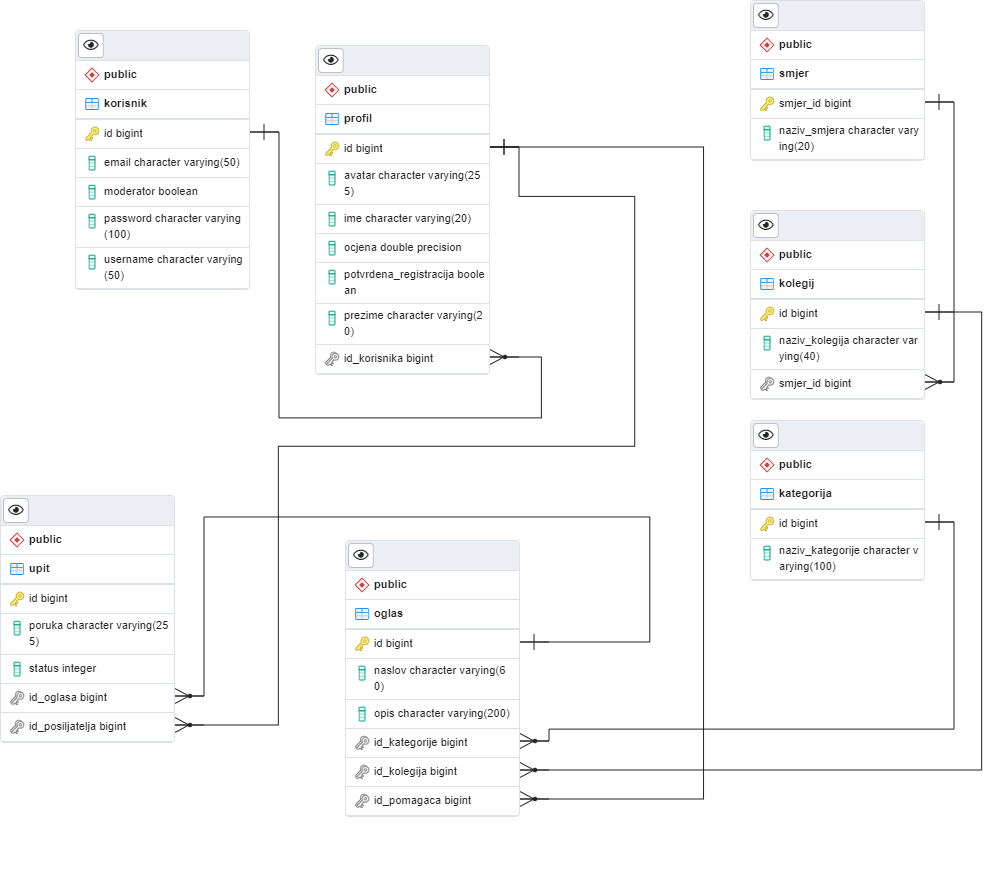
\includegraphics[scale=0.6]{dijagrami/baza.png}
					\centering
					\caption{Dijagram baze podataka}
					\label{fig:dijagram baze}
				\end{figure}
				
			\eject
			
			
		\section{Dijagram razreda}
		
			Na slikama \ref{fig:cont}, \ref{fig:DAO} i \ref{fig:models} prikazani su razredi koji pripadaju backend dijelu MVC arhitekture. Razredi su podijeljeni u tri dijela: Controllers, DAO i Modele. Razredi u Controllers dijelu nasljeđuju razred Controller i upravljaju pristiglim zahtjevima na backend dio aplikacije. Metode implementirane u tim razredima manipuliraju s DAO (Dana Access Object) razredima. DAO razredi su modelirani i dohvaćeni pomoću metoda koje su implentirane u Model razredima. Povratne vrijednosti metoda u Controller razredima su JSON datoteke s HTML status kodom.
			
			Zbog lakšeg prikaza i organizacije, razredi su logički podijeljeni po pravu pristupa metodama određenih aktora te su prikazane samo ovisnosti između razreda koji pripadaju istom dijelu dijagrama. Iz naziva i tipova atributa u razredima može se zaključiti vrsta ovisnosti među različitim razredima.
			
			\begin{figure}[H]
				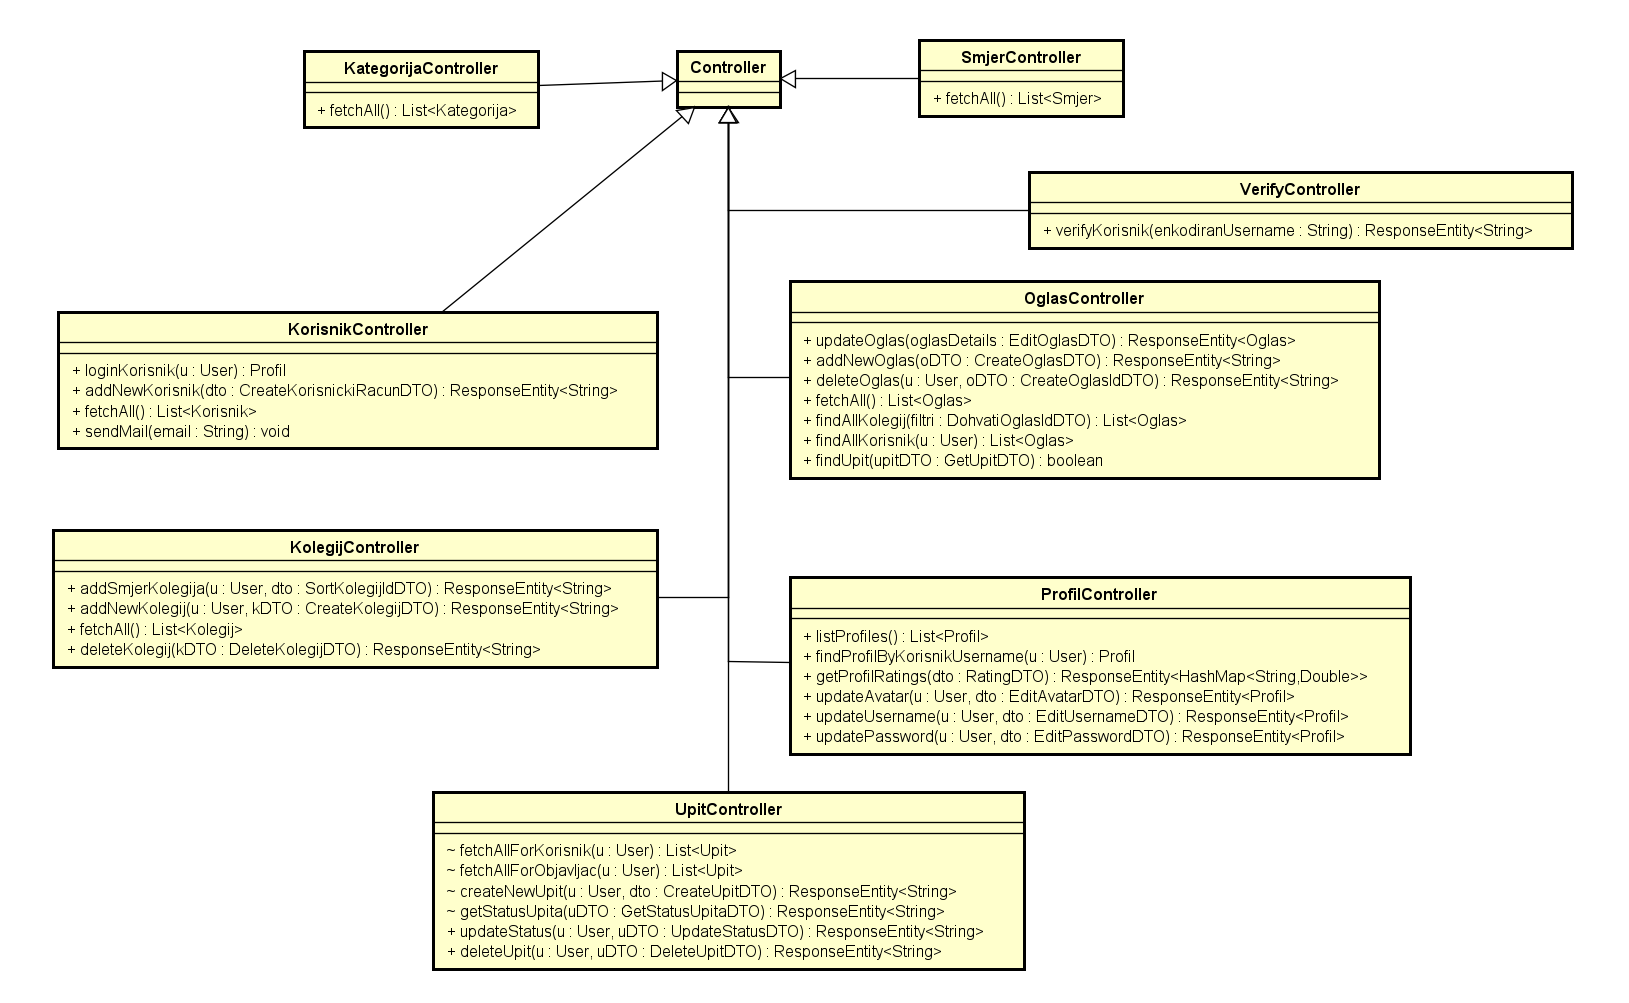
\includegraphics[scale=0.35]{dijagrami/dijagram_razreda_controllers.png}
				\centering
				\caption{Dijagram razreda - Controllers}
				\label{fig:cont}
			\end{figure}
		
			\begin{figure}[H]
				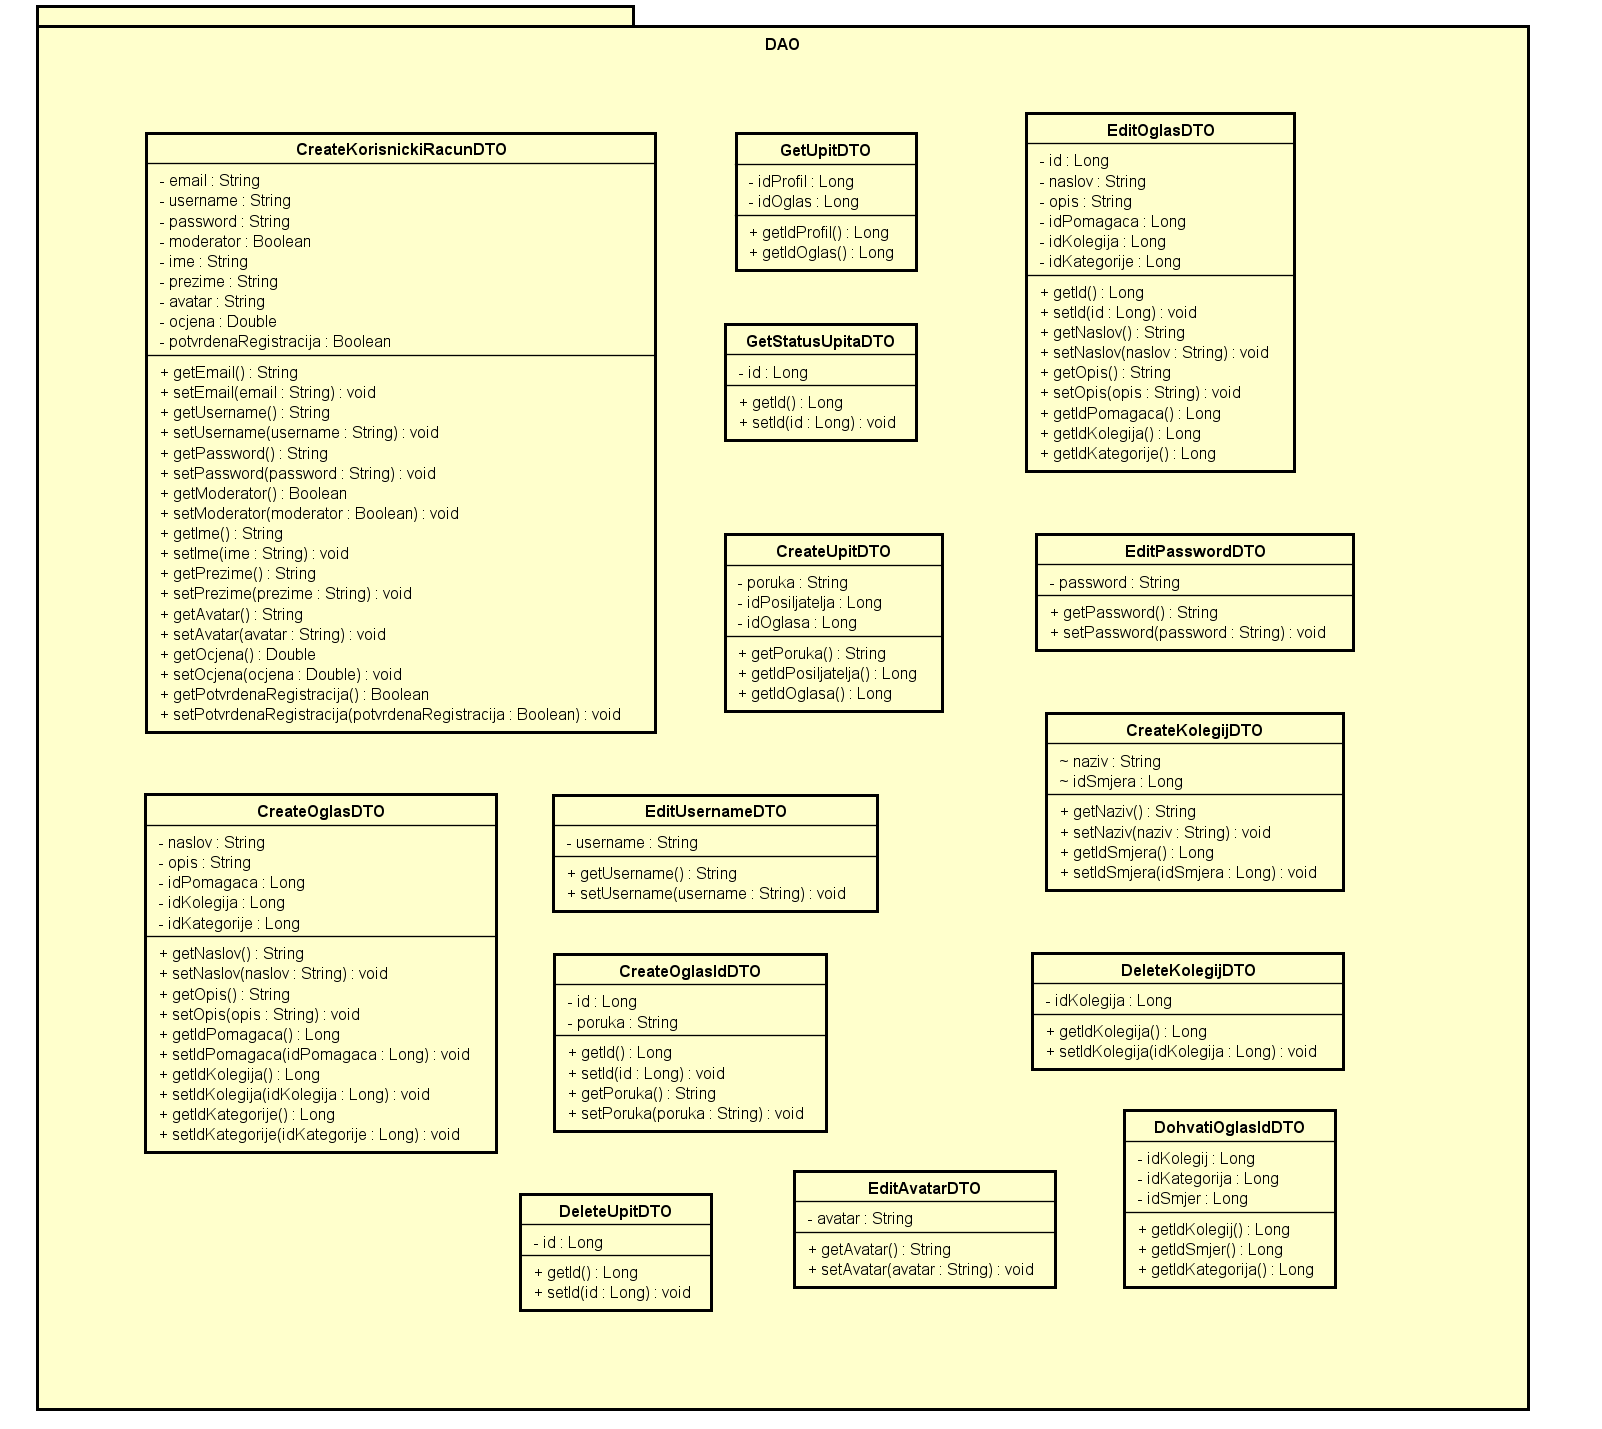
\includegraphics[scale=0.37]{dijagrami/dijagram_razreda_DAO.png}
				\centering
				\caption{Dijagram razreda - Dana Access Object}
				\label{fig:DAO}
			\end{figure}
			
			Razredi modela preslikavaju strukturu baze podataka u aplikaciju. Implementirane metode komuniciraju s bazom te vraćaju tražene podatke. Razred Korisnik predstavlja registriranog korisnika i njegovo osnovne informacije važne za prijavu i slanje e-maila: e-mail adresa, korisničko ime i zaporka. Razred Profil sadrži više dodatnih informacija o registriranom korisniku kao što su ime, prezime, odabrani avatar i status je li registracija potvrđena putem maila ili nije. Razred Smjer predstavlja dostupne smjerove na studiju. Razred Kolegij sadrži informacije o kolegijima koji su dodani u bazu. Dostupne informacije su naziv kolegija i smjer kojem taj kolegij pripada. Razred Kategorija predstavlja kategoriju u koju možemo svrstati oglas. U sustavu postoji 5 različitih kategorija: laboratorijska vježba, blic, gradivo, kontinuirani ispit i ispitni rok. Razred Oglas predstavlja informacije koje se pohranjuju u bazu za pojedini oglas, a to su: naziv oglasa, opis oglasa, kolegij za koji se oglas objavljuje, kategorija kojoj oglas pripada i profil koji je poslao upit za taj oglas. Razred Upit pamti podatke vezane uz javljanje na određeni oglas. Sadrži oglas za koji se šalje upit, sadrži profil koji stvara upit, poruku s kojom korisnik šalje upit i status u kojem se nalazi upit. Razred StatusUpita predstavlja enumeraciju pomoću koje se modelira jedan od 3 stanja upita: u tijeku, prihvaćen i odbijen.
			
			\begin{figure}[H]
				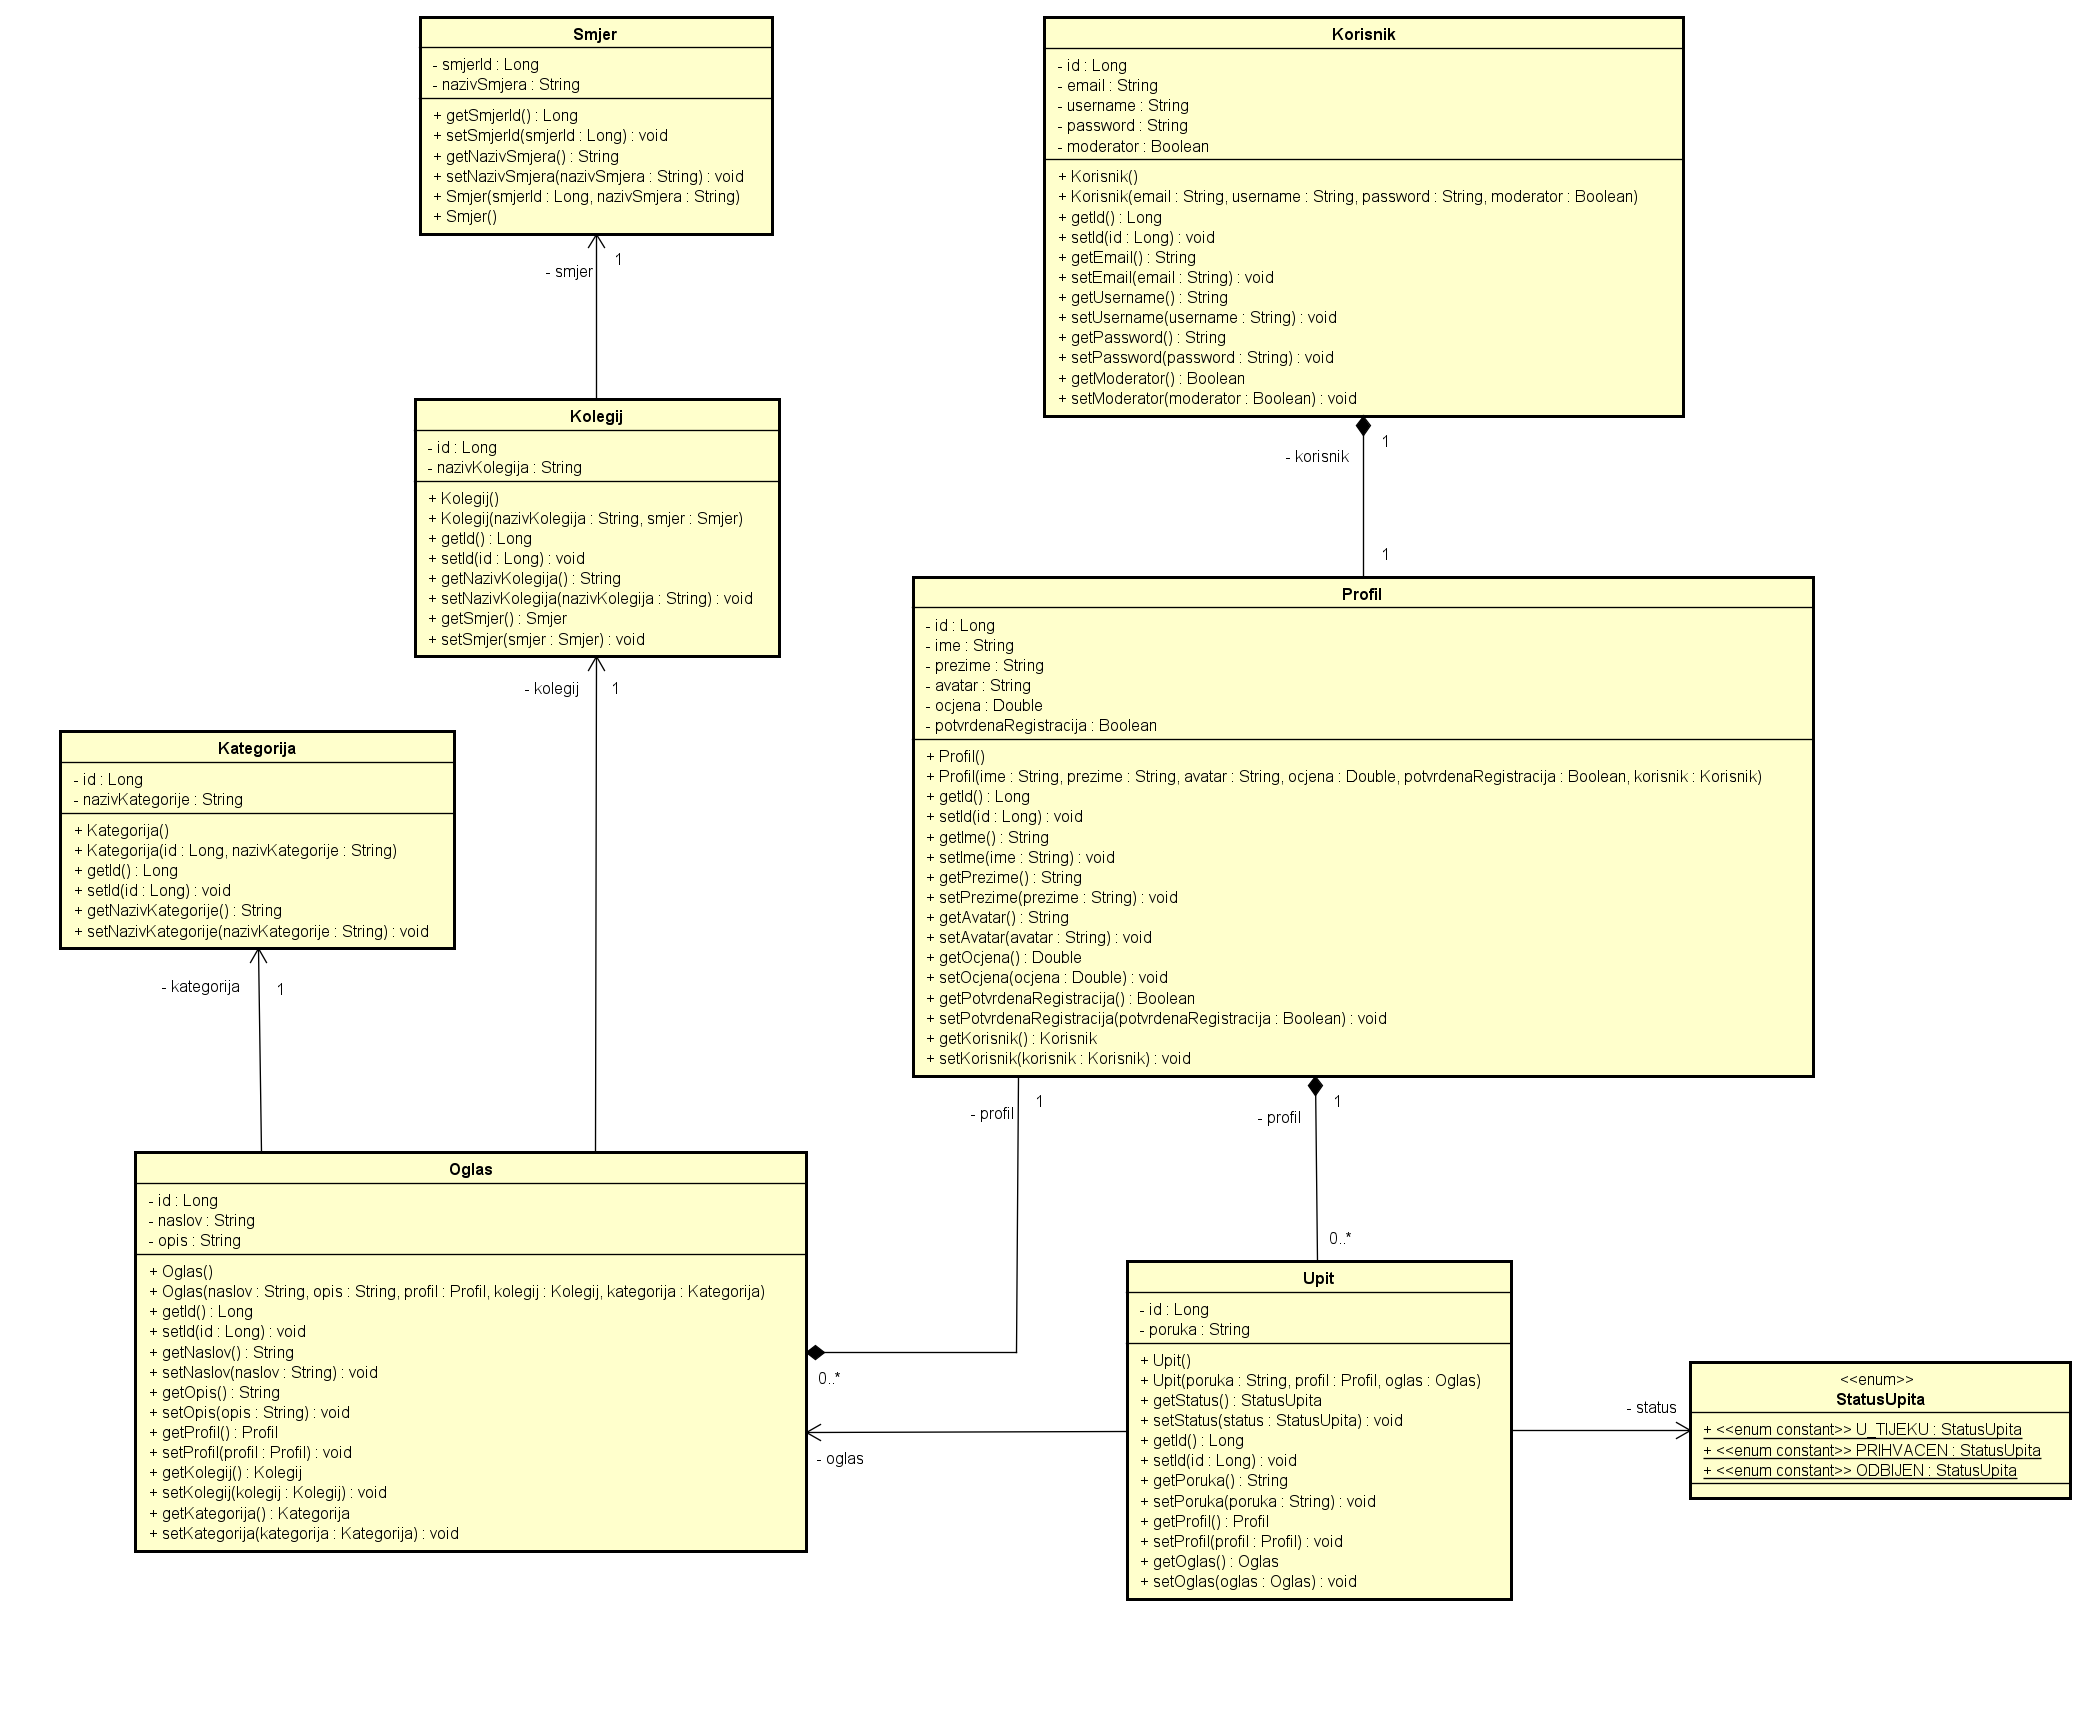
\includegraphics[scale=0.28]{dijagrami/dijagram_razreda_models.png}
				\centering
				\caption{Dijagram razreda - Models}
				\label{fig:models}
			\end{figure}
		
			\eject
		\section{Dijagram stanja}
			Na slici \ref{fig:dijagram stanja} prikazan je dijagram stanja. On prikazuje dinamičko ponašanje dijela sustava. Dijagram opisuje stanja za registriranog korisnika. Korisnik nakon prijave dolazi na početnu stranicu. Tamo ima mogućnost stvaranja novog oglasa, javljanja na tuđe oglase, filtriranja po smjeru, kolegiju i kategoriji te odlazak na stanicu „Profile“. Na stranici profila korisnik ima mogućnost uređivanja svojih podataka, tj. mijenjanja avatara, lozinke i nadimka. Ako postoji upit na oglas koje je napisao korisnik, onda korisnik ima mogućnost prihvatiti ili odbiti taj upit. U dijelu „Moji objavljeni oglasi“ korisnik ima mogućnost uređivanja oglasa, klikom na ikonu olovke, ili brisanja oglasa, klikom na ikonu smeća. Korisnik iz svih stanja može doći u stanje početne stranice i stranice profila te se iz svih stanja može odjaviti.
		
			\begin{figure}[H]
				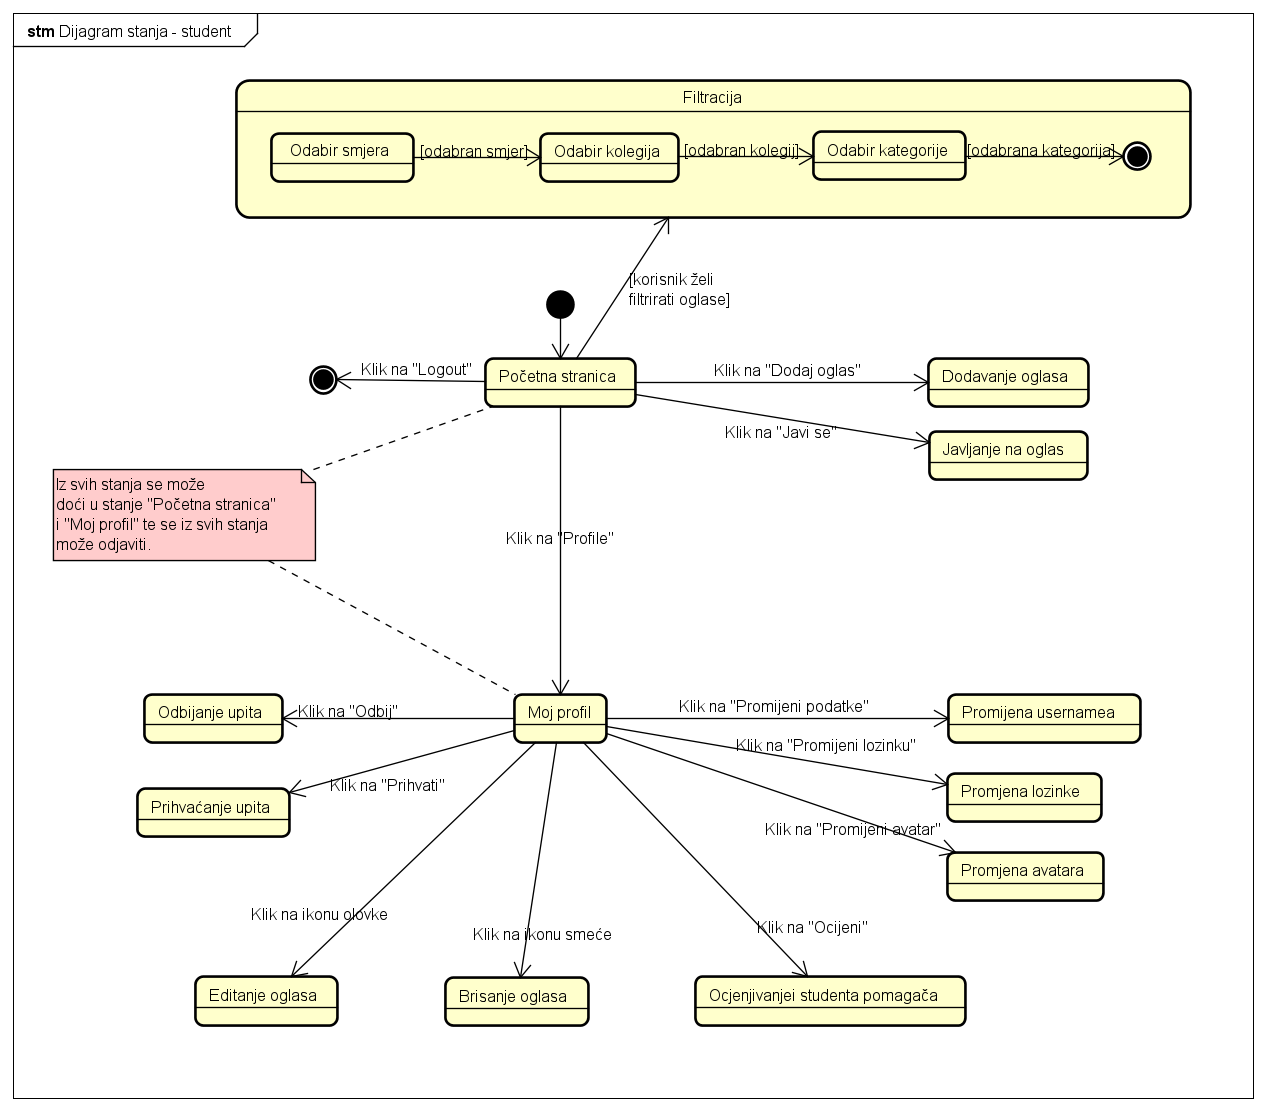
\includegraphics[scale=0.45]{dijagrami/DijagramStanja.png}
				\centering
				\caption{Dijagram stanja}
				\label{fig:dijagram stanja}
			\end{figure}
			
			\eject 
		
		\section{Dijagram aktivnosti}
			Dijagram aktivnosti koristi se za modeliranje poslovnih procesa ili upravljačkog i podatkovnog toka. Na slici \ref{fig:dijagram aktivnosti} prikazan je dijagram aktivnosti registriranog korisnika. Korisnik nakon prijave stvara novi oglas nakon čega preko e-maila dobiva upit na stvoreni oglas. Korisnik odabire hoće li prihvatiti ili obiti upit na oglas. Zatim se korisnik javlja na oglas nekog drugog studenta pomagača te nakon potvrđenog upita na oglas ocjenjuje instrukcije. Na posljetku korisnik briše svoj oglas te se odjavljuje.
			
			\begin{figure}[H]
				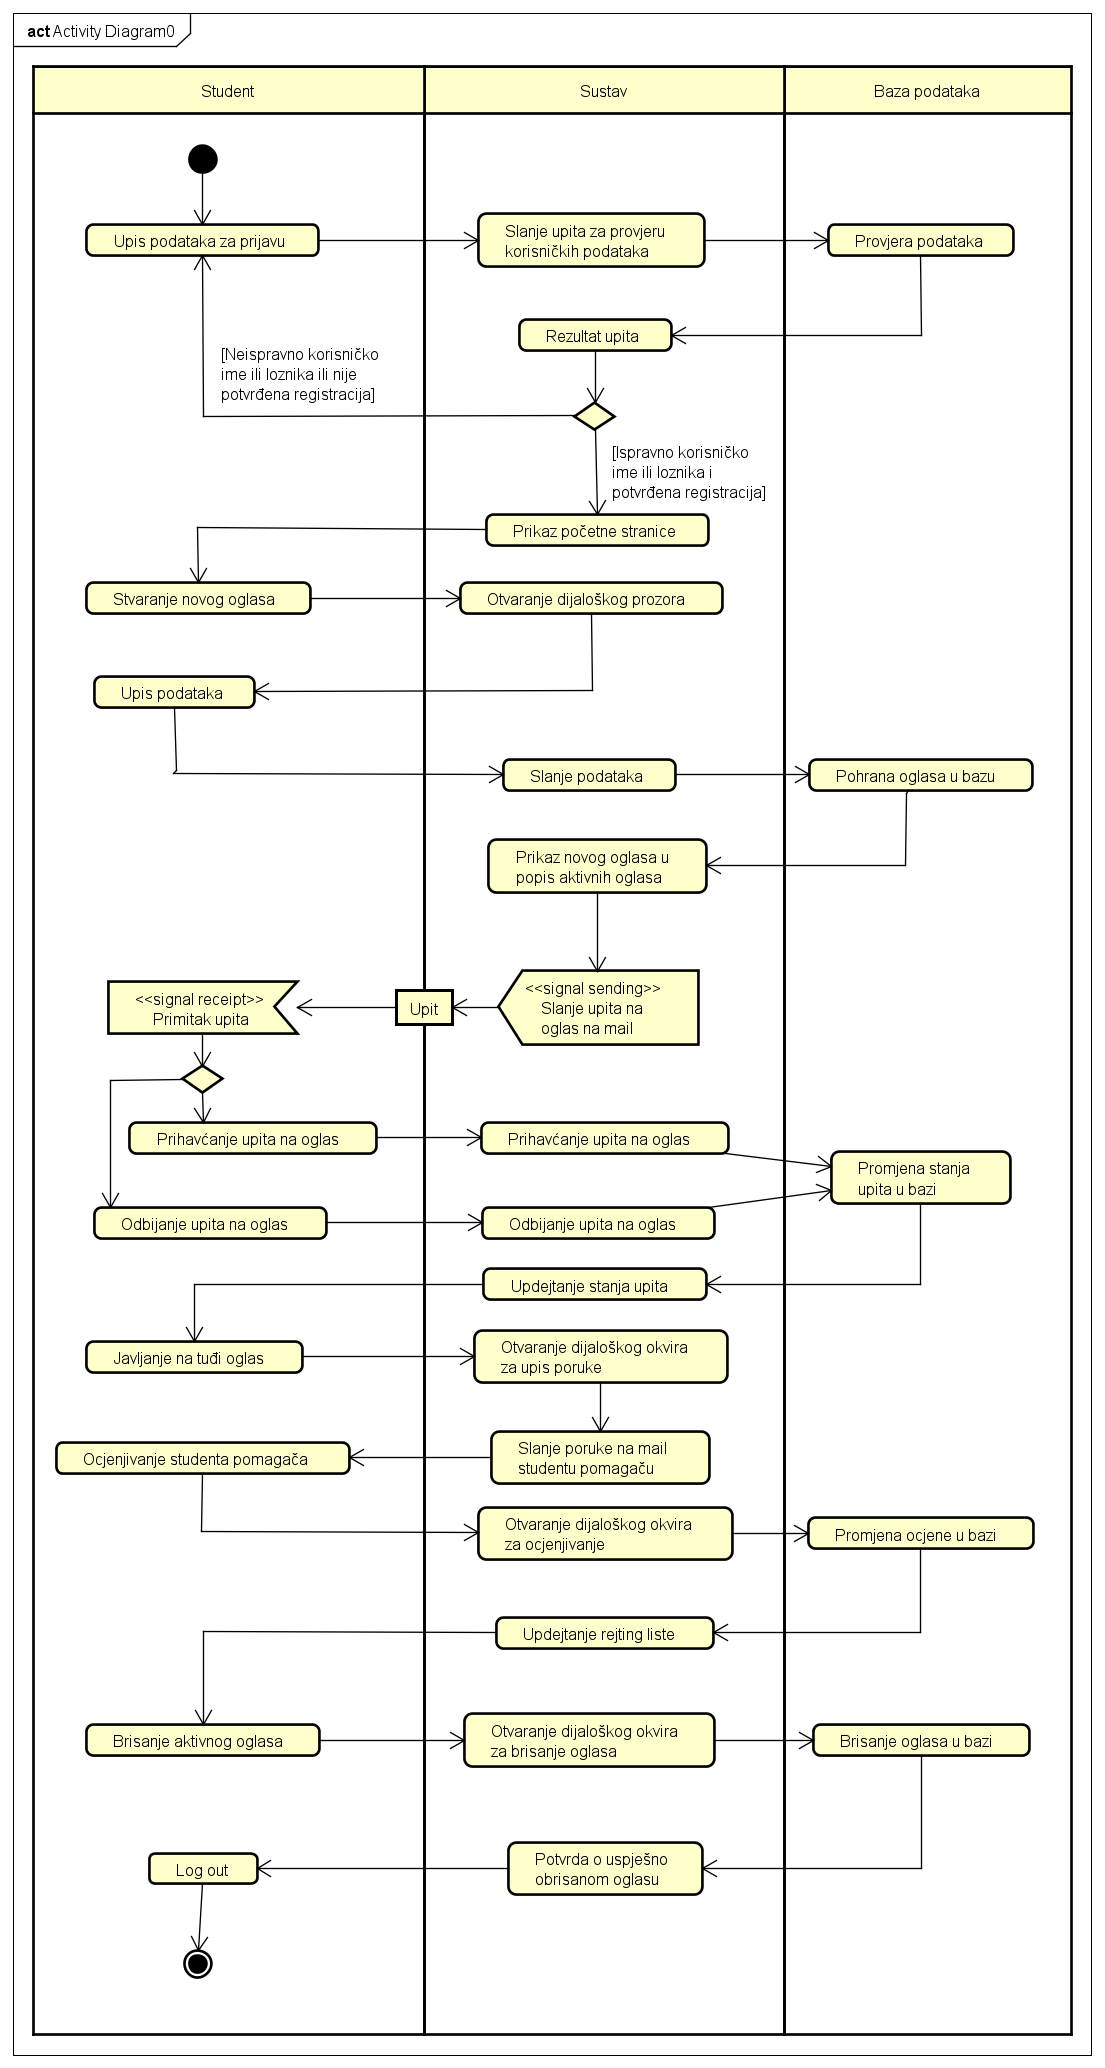
\includegraphics[scale=0.42]{dijagrami/DijagramAktivnosti.png}
				\centering
				\caption{Dijagram aktivnosti}
				\label{fig:dijagram aktivnosti}
			\end{figure}
			
			\eject
			
		\section{Dijagram komponenti}
		Dijagram komponenti prikazan na slici \ref{fig:dijagram konponenti} opisuje međusobnu ovisnost komponenti, internu strukturu komponenti i njihov odnos prema okolini. Sustavu se pristupa preko dva sučelja. Prvo sučelje služi za dohvat HTML, CSS i JS datoteka. To sučelje pripada frontend dijelu aplikacije. Router je komponenta koja na temelju url određuje koje datoteke će sučelje vratiti kao rezultat upita. Frontend dio aplikacije sastoji se od niza JavaScript datoteka koje su raspoređene u logičke cjeline. Te logičke cjeline nazvane su po različitim tipovima aktora koji pristupaju aplikaciji. Sve JavaScript datoteke u logičkim cjelinama ovise o React biblioteci pomoću koje se dohvaćaju gotove komponente kao što su polja za upis podataka, gumbi, odlomci, itd. Drugo sučelje pomoću kojeg se može pristupiti aplikaciji je sučelje koje služi za dohvat JSON podataka. Preko tog sučelja pristupa se REST API komponenti sustava. REST API poslužuje podatke koji pripadaju backend dijelu aplikacije. Hibernate je implementacija JPA putem kojeg se pomoću SQL upita može pristupiti i dohvatiti podatke iz baze podataka. Tako dohvaćeni podaci iz baze šalju se dalje MVC arhitekturi u obliku DAO (Data Access Object). React-view je komponenta koja preko dostupnih sučelja komunicira sa Sinappsa aplikacijom te ovisno o korisnikovim akcijama osvježava prikaz i dohvaća nove podatke od aplikacije.  
		
		\begin{figure}[H]
			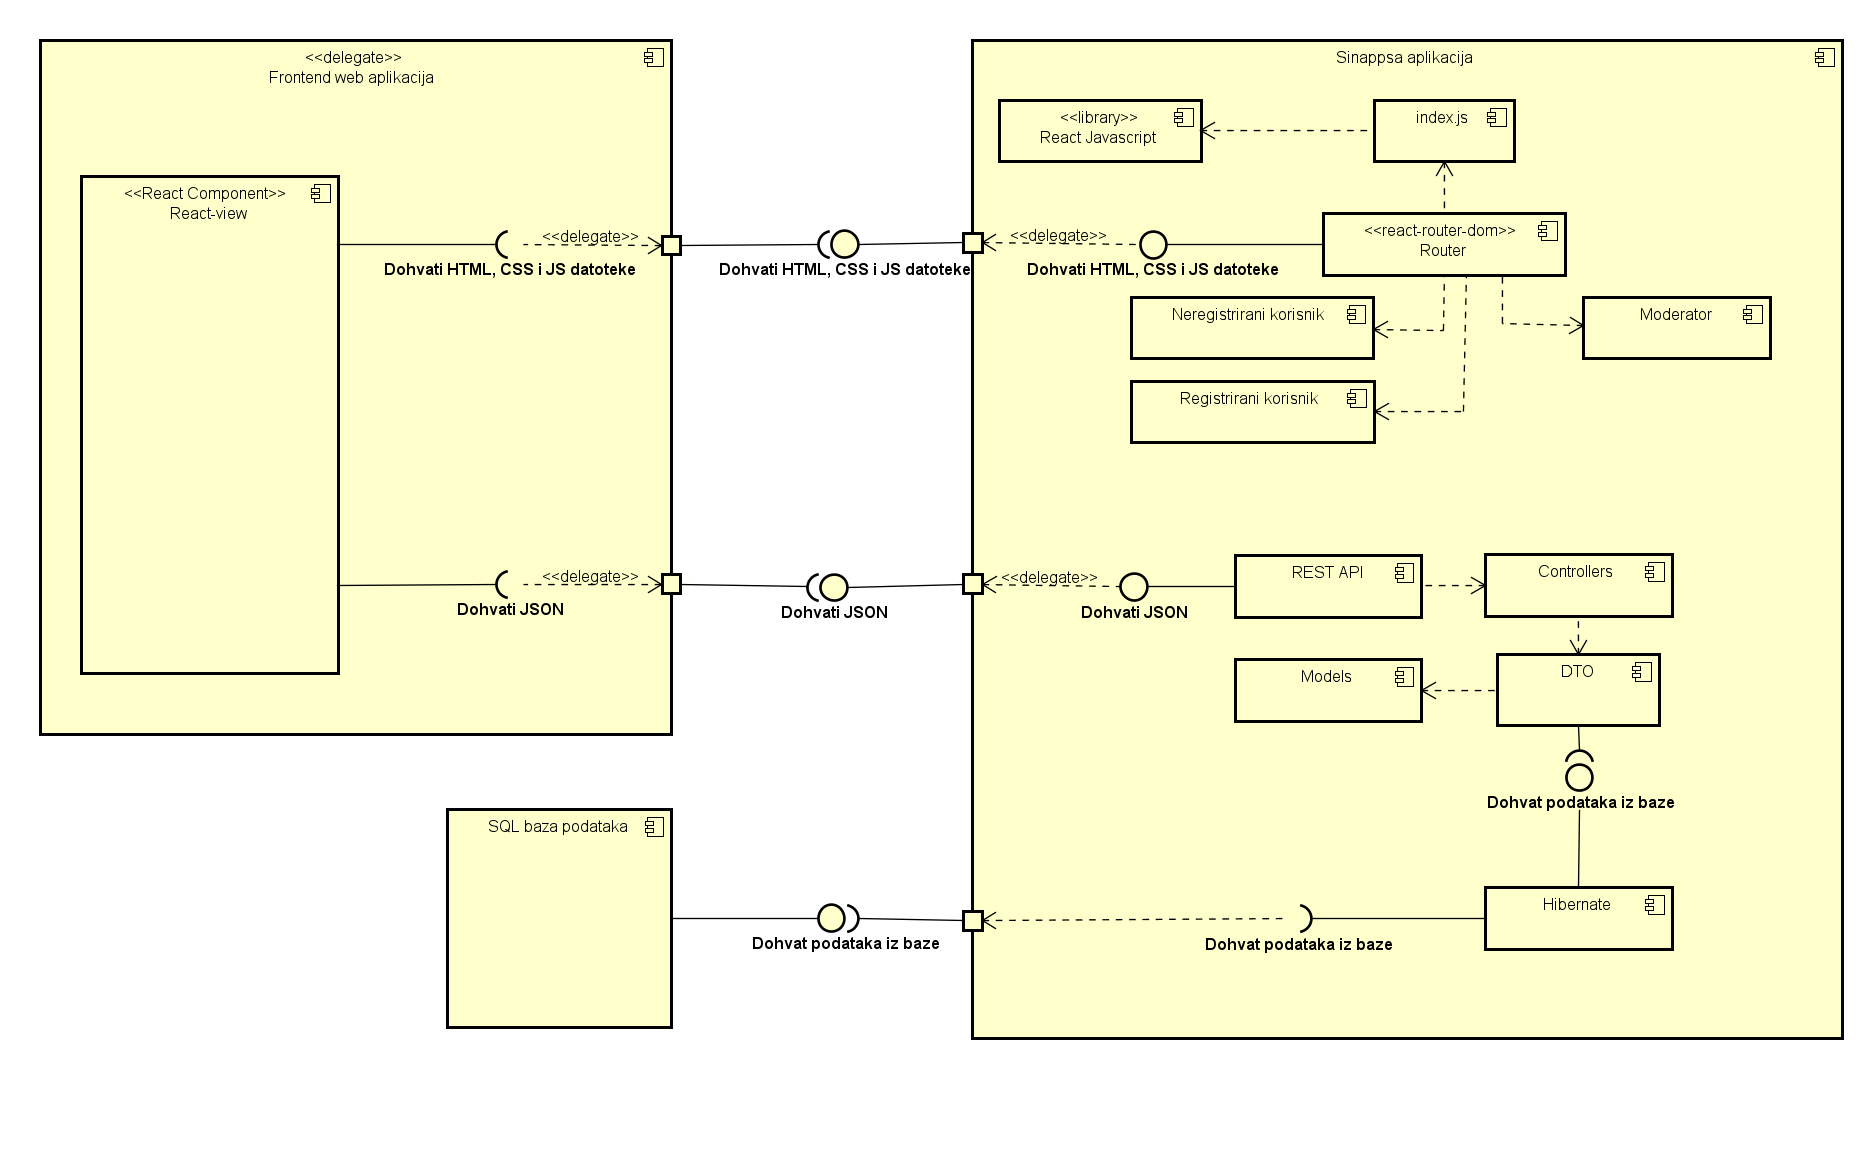
\includegraphics[scale=0.31]{dijagrami/dijagram_komponenti.png}
			\centering
			\caption{Dijagram komponenti}
			\label{fig:dijagram konponenti}
		\end{figure}
		